
\subsection{Stabilność}
\begin{frame}{Stabilność}
  \begin{block}{Powód:}
\begin{itemize}
    \item $ 0  \le t \leq \alpha $
    \item $\text{wybór } \Delta t $
\end{itemize}
  \end{block}
    
      $\Delta x = h $ \\
      $\Delta t = k$ \\
      $ R = \{P(x,t): 0 < x < a, t > 0\}$ \\
      $S - \text{boundary of R}$ \\
      $R_h = x \rightarrow \text{interior points}$ \\
      $S_h = 0 \rightarrow \text{boundary points}$
  \end{frame}

\begin{frame}
  \centerline{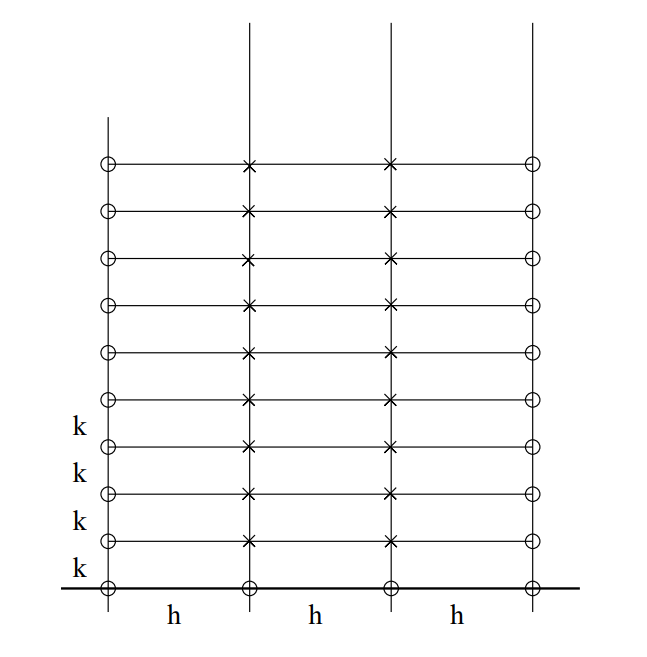
\includegraphics[height = 0.85 \textheight]{img/23/stabilnosc}}
\end{frame}

\begin{frame}
$ m^{th} \text{ row of grid points:}$
$$y = m \cdot k$$
\centerline{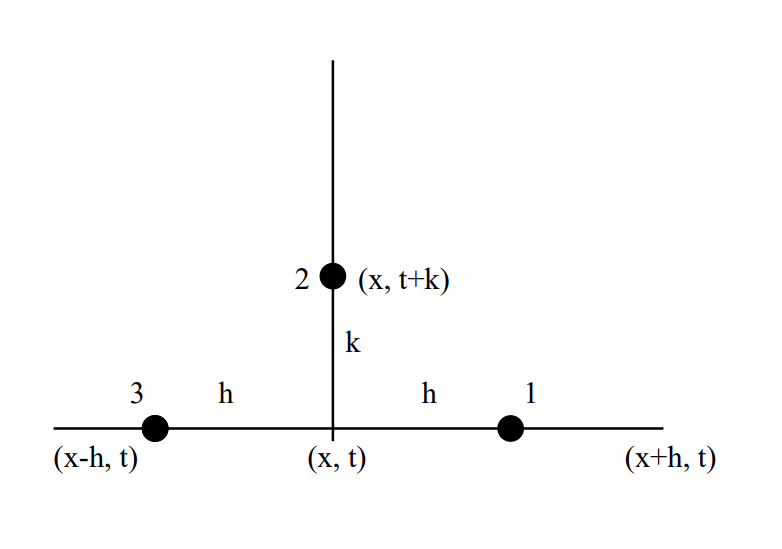
\includegraphics[height = 0.55 \textheight]{img/23/stabilnosc2}}

\begin{block}{}
   $$ \begin{array}{l}
   u_{xx}(x,t) = \frac{u(x-h,t)-2 \cdot u(x,t) + u(x+h,t)}{h^{2}}, \\ \\
   u_t (x,t)= \frac{u(x,t+k)-u(x,t)}{k}
   \end{array}$$
 \end{block}

\end{frame}

\begin{frame}
Po podstawieniu do (\ref{7}) i uporządkowaniu:
$$u(x,t+k) = u(x,t) + \frac{k}{h^2}[u(x+h,t)-2\cdot u(x,t)+u(x-h,t)]$$
wprowadzając: $\lambda = \frac{k}{h^2}$, uzyskujemy:
$$u(x,t+k) = \lambda \cdot u(x+h,t)+(1-2\lambda)u(x,t)+\lambda \cdot u(x-h,t)$$
używając oznaczeń z rysunku:
$$u_2 = \lambda \cdot u_1+(1-2\lambda)\cdot u_0+\lambda \cdot u_3$$


$$ \textcolor{blue}{\text{Algorytm (Explicit Method):}}\left
\{ \begin{array}{lrl}
       \text{konstrukcja siatki}\\
       \text{wiersz po wierszu} \rightarrow \text{kolejno w górę.}
        \end{array} \right. $$
\end{frame}

\begin{frame}
Rozwiązania $\rightarrow$ mają własność min-max (physically reasonable)
\center{stable if any only if is physically reasonable}
\centerline{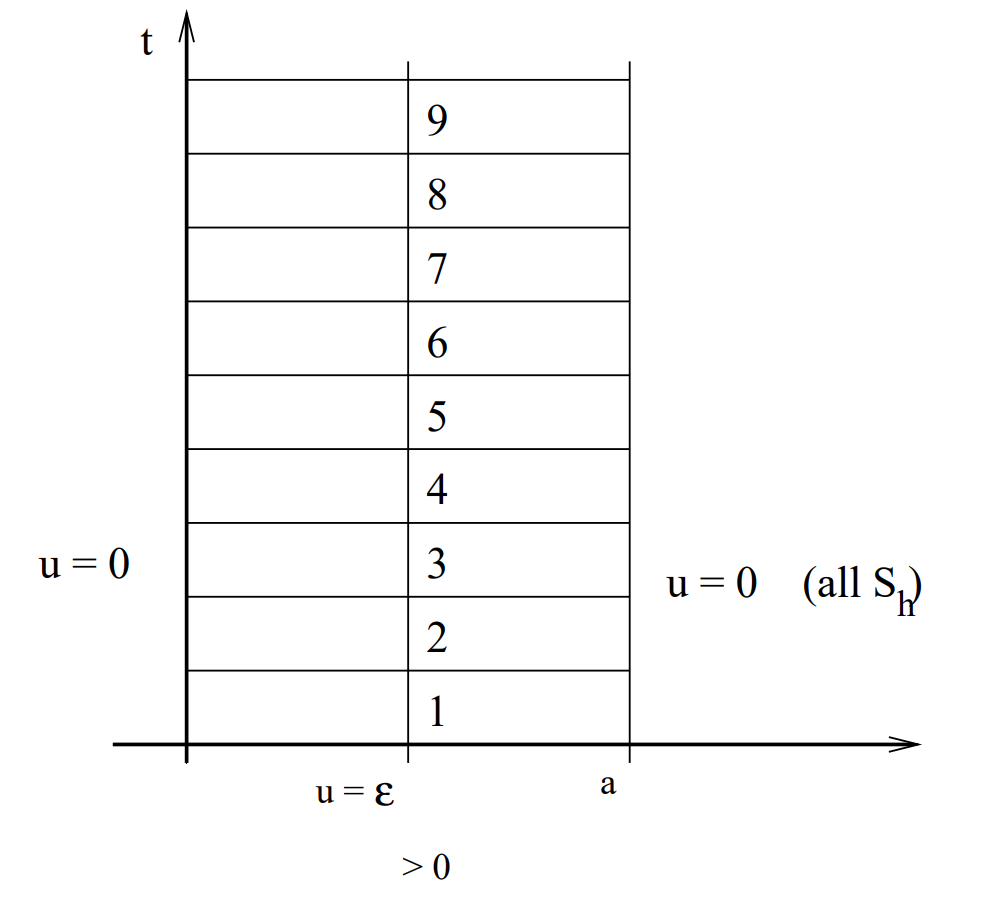
\includegraphics[height = 0.70 \textheight]{img/23/stabilnosc4}}
\end{frame}

\begin{frame}
$\Delta x = \frac{a}{2} , \quad \Delta t = k$ \\
\vspace{5mm}
$u_1 = (1 - 2 \lambda)\varepsilon ,    u_2 = (1 - 2\lambda )^2\varepsilon , u_3 = (1-2\lambda)^3 \cdot \varepsilon , ... u_m = (1-2\lambda)^m\cdot \varepsilon$ \\
\vspace{5mm}
$\ 0 \leq u \leq \varepsilon  \quad \text{na} \ S_n$
$$0 \leq (1-2 \lambda)^m \cdot \varepsilon \leq \varepsilon$$
$\Longrightarrow 0 \leq \lambda \leq \frac{1}{2}$
\end{frame}